\section*{Learning Objectives}

\begin{itemize}
\item Establish key definitions for fields, vectors, vector spaces, linear combinations, linear independence, subspaces, basis vectors, linear operators, matrix representations, eigenvalues and eigenvectors.
\item Initial practice with the proof techniques of the previous chapter.
\end{itemize}

\section*{Outcomes} 
\begin{itemize}
\item Understand a very general notion of vector spaces, where the vectors range from the standard column vectors in $\real^n$ to matrices and functions.

\item Understand how the notion of representing a vector with respect to a set of basis vectors establishes one-to-one relations with columns of numbers that can be used in numerical computations.

\item Understand a related notion for associating linear operators to matrices.

\item Set you up for Chapter 3 which solves best approximation problems for generalizations of the Euclidean norm.

\item Have your mind blown by the real numbers forming an infinite dimensional vector space over the field of rational numbers. 


\end{itemize}

\newpage

\section{Fields and Vector Spaces}

Mostly in this course, we work with the real numbers or the complex numbers. However, in this Chapter, as part of our push to tear you away from the familiar and confront you with more abstraction than you may have seen before, we define a general \emph{field}, ${\cal F}$. When you are first learning the abstract definition, it is good to keep a `` canonical example'' in mind, and that would be ${\cal F} = \real$.\\


\begin{definition} (Chen, 2nd edition, page 8) : A \textbf{field} consists of a set, denoted by $\mathcal{F}$, of elements called \textbf{scalars} and two operations called addition ``$+$'' and multiplication ``$\cdot$''; the two operations are defined over $\mathcal{F}$ such that they satisfy the following conditions:
    \begin{enumerate}
        \item To every pair of elements $\alpha$ and $\beta$ in $\mathcal{F}$, there correspond an element $\alpha+\beta$ in $\mathcal{F}$ called the \emph{sum} of $\alpha$ and $\beta$, and an element $\alpha \cdot \beta$ (or simply $\alpha \beta$) in $\mathcal{F}$ called the \emph{product} of $\alpha$ and $\beta$.
        \item Addition and multiplication are respectively commutative: For any $\alpha$ and $\beta$ in $\mathcal{F}$,
        \begin{align*}
            \alpha+\beta &= \beta + \alpha & \alpha\cdot\beta &= \beta\cdot\alpha
        \end{align*}
        \item Addition and multiplication are respectively associative: For any $\alpha$, $\beta$, $\gamma$ in $\mathcal{F}$,
        \begin{align*}
            \left(\alpha+\beta\right)+\gamma &= \alpha + \left(\beta+\gamma\right) & \left(\alpha\cdot\beta\right)\cdot\gamma = \alpha\cdot\left(\beta\cdot\gamma\right)
        \end{align*}
        \item Multiplication is distributive with respect to addition: For any $\alpha$, $\beta$, $\gamma$ in $\mathcal{F}$,
        \begin{align*}
            \alpha\cdot\left(\beta+\gamma\right) = \left(\alpha\cdot\beta\right)+\left(\alpha\cdot\gamma\right)
        \end{align*}
        \item $\mathcal{F}$ contains an element, denoted by $0$, and an element, denoted by $1$, such that $\alpha + 0 = \alpha$ and $1\cdot\alpha = \alpha$ for every $\alpha$ in $\mathcal{F}$.
        \item To every $\alpha$ in $\mathcal{F}$, there is an element $\beta$ in $\mathcal{F}$ such that $\alpha+\beta = 0$. The element $\beta$ is called the \emph{additive inverse}.
        \item To every $\alpha$ in $\mathcal{F}$ which is not the element 0, there is an element $\gamma$ in $\mathcal{F}$ such that $\alpha\cdot\gamma = 1$. The element $\gamma$ is called the \emph{multiplicative inverse}.
    \end{enumerate}
\end{definition}

\vspace*{.2cm}
To show a given set is a field, you must check all seven axioms. To show something is not a field, you only need to show that one of the axioms fails.      
\vspace*{.2cm}

\begin{center}
\begin{tabular}{|c|l|}
\hline
Examples of Fields& Non-examples \\ \hline
$\real$ & Irrational (Fails axiom 1) \\ \hline
$\cp$ & $2\times2$ matrices, real coeff. (Fails axiom 2) \\ \hline
$\mathbb{Q}$ & $2\times2$ diagonal matrices real coeff. (Fails axiom 7) \\ \hline
\end{tabular}
\end{center}

\vspace*{,2cm}

\begin{definition} (Chen 2nd Edition, page 9) A \textbf{vector space (or, linear space)} over a field $\mathcal{F}$, denoted by $\left(\mathcal{X},\mathcal{F}\right)$, consists of a set, denoted by $\mathcal{X}$, of elements called \textbf{vectors}, a field $\mathcal{F}$, and two operations called \textbf{vector addition} and \textbf{scalar multiplication}. The two operations are defined over $\mathcal{X}$ and $\mathcal{F}$ such that they satisfy all the following conditions:
    \begin{enumerate}
        \item To every pair of vectors $v^1$ and $v^2$ in $\mathcal{X}$, there corresponds a vector $v^1+v^2$ in $\mathcal{X}$, called the sum of $v^1$ and $v^2$ \footnote{We use superscripts $v^1, v^2, v^3$ to denote different \emph{vectors}. The superscripts \emph{do not} denote powers.}.
        \item Addition is commutative: For any $v^1,v^2$ in $\mathcal{X}$, $v^1+v^2 = v^2+v^1$.
        \item Addition is associative: For any $v^1,v^2$, and $v^3$ in $\mathcal{X}$, $\left(v^1+v^2\right)+v^3 = v^1 + \left(v^2+v^3\right)$.
        \item $\mathcal{X}$ contains a vector, denoted by \textbf{0}, such that \textbf{0}$ + v = v$ for every $v$ in $\mathcal{X}$. The vector \textbf{0} is called the zero vector or the origin.
        \item To every $v$ in $\mathcal{X}$, there is a vector $\bar v$ in $\mathcal{X}$, such that $v + \bar v = 0$.
        \item To every $\alpha$ in $\mathcal{F}$, and every $v$ in $\mathcal{X}$, there corresponds a vector $\alpha\cdot v$ in $\mathcal{X}$ called the \emph{scalar product} of $\alpha$ and $v$.
        \item Scalar multiplication is associative: For any $\alpha, \beta$ in $\mathcal{F}$ and any $v$ in $\mathcal{X}$, $\alpha\cdot\left(\beta\cdot x\right) = \left(\alpha\cdot\beta\right)\cdot v$.
        \item Scalar multiplication is distributive with respect to vector addition: For any $\alpha$ in $\mathcal{F}$ and any $v^1,v^2$ in $\mathcal{X}$, $\alpha\cdot\left(v^1+v^2\right) = \alpha\cdot v^1 + \alpha\cdot v^2$.
        \item Scalar multiplication is distributive with respect to scalar addition: For any $\alpha ,\beta$ in $\mathcal{F}$ and any $v$ in $\mathcal{X}$, $\left(\alpha+\beta\right)\cdot v = \alpha\cdot v + \beta\cdot v$.
        \item For any $v$ in $\mathcal{X}$, $1\cdot v=v$, where $1$ is the element $1$ in $\mathcal{F}$.
    \end{enumerate}
        
\end{definition} 

\vspace*{.2cm}

\begin{example} 
 $\mathcal{F} = $ field, $\mathcal{X} = $ set of vectors
    \begin{enumerate}
        \item Every field forms a vector space over itself. $\left(\mathcal{F},\mathcal{F}\right)$. Examples: $\left(\real,\real\right)$, $\left(\cp,\cp\right)$, $\left(\mathbb{Q},\mathbb{Q}\right)$.
        \item $\left(\cp,\real\right)$, meaning $\mathcal{X} = \cp$, $\mathcal{F} = \real$, is a vector space. This works because a real scalar $\alpha \in \mathcal{F}=\real$ times a complex number $v \in \mathcal{X}=\cp$ yields a complex number $\alpha \cdot v \in \mathcal{X}=\cp$. 
        \item $\mathcal{F} = \real$, and $\mathcal{X} = \left\{f:D\to\real\right\} = \left\{\mbox{functions from } D \mbox{ to } \real \right\}$, where $D \subset \real$ (examples: $D = \left[a,b\right]; D = \left(0,\infty\right); D = \real$) with vector addition and scalar times vector multiplication defined as follows:
        \begin{enumerate}
            \item $\forall~ f,g\in\mathcal{X}$, define $f+g \in \mathcal{X}$ by $\forall t\in D,\ \left(f+g\right)(t) := f(t) + g(t)$;
            \item  $\forall~ f \in\mathcal{X}$ and $\alpha\in\real$, define $\alpha\cdot f\in\mathcal{X}$ by $\forall t\in D, \left(\alpha\cdot f\right)(t) := \alpha\cdot f(t)$.
            \end{enumerate}
            Note that we are using the known properties of addition and multiplication of real numbers to define what we mean by the sum of two functions and the product of a real number and a function. To prove that $(\mathcal{X}, \mathcal{F})$ is a vector space, you must check all ten of the axioms. We'll check \#8 to illustrate what as to be done: we need to show that  scalar multiplication is distributive with respect to vector addition: 
            $$\alpha \cdot (f + g) = \alpha \cdot f + \alpha \cdot g.$$ 
            Our method of proof is to show that the left hand side (LHS) equals the right hand side (RHS) when 
            \begin{itemize}
                \item we use the definition of a function evaluated at a point $t$, and
                \item we subsequently apply the known definitions for sums and products of real numbers.
            \end{itemize}
            Let $t \in D$, then 
               \begin{enumerate}
            \item LHS: $[\alpha \cdot (f+g)](t): = \alpha \cdot[f + g](t) = \alpha \cdot [f(t) + g(t)] = \alpha \cdot f(t) + \alpha \cdot g(t)$.
            \item RHS: $[\alpha \cdot f + \alpha \cdot g](t):= [\alpha \cdot f](t) + [ \alpha \cdot g](t) = \alpha \cdot f(t) + \alpha \cdot g(t)$
            \item Hence, LHS = RHS and we are done.
            \end{enumerate}
        \item Let $\mathcal{F}$ be a field and define $\mathcal{X}:=\mathcal{F}^n$ the set of n-tuples written as columns
        \begin{align*}
            \mathcal{F}^n: = \left\{\left.\begin{bmatrix} \alpha_1 \\ \vdots \\ \alpha_n \end{bmatrix} \right| \alpha_i \in \mathcal{F}, 1 \leq i \leq n\right\}
        \end{align*}
        Then $(\mathcal{F}^n, \mathcal{F})$ is a vector space with the operations
        \begin{enumerate}
            \item Vector Addition: $\begin{bmatrix} \alpha_1 \\ \vdots \\ \alpha_n \end{bmatrix} + \begin{bmatrix} \beta_1 \\ \vdots \\ \beta_n \end{bmatrix} = \begin{bmatrix} \alpha_1 + \beta_1 \\ \vdots \\ \alpha_n + \beta_n \end{bmatrix}$
            \item Scalar Multiplication: $\alpha\cdot x = \begin{bmatrix} \alpha x_1 \\ \vdots \\ \alpha x_n \end{bmatrix}$
        \end{enumerate}
        \item In a similar manner, one can take $\mathcal{X} := \mathcal{F}^{n\times m} = \left\{n\times m \mbox{ matrices with coefficients in } \mathcal{F}\right\}$ with vector addition and scalar times vector multiplication defined in the obvious ways. Hence, matrices can be viewed as vectors. 
        
        \item $(\real,\mathbb{Q})$ is a vector space. It is not particular useful in Robotics. It's kind of cool to think about. The set of vectors is $\real$. Clearly, the sum any two real numbers is again a real number, and hence a vector. The usual scalar times vector multiplication works because the product of a rational number and a real number is a real number, and hence is a vector. 
    \end{enumerate}
    \end{example}

\vspace*{.2cm}

    \begin{nonexample} \mbox{ }
    \begin{enumerate}
        \item Take $ \mathcal{X} = \real, \mathcal{F} = \cp$. Then $(\mathcal{X}, \mathcal{F}):=\left(\real,\cp\right) $ fails the definition of scalar multiplication (and others).
        \item $ \mathcal{X} = \left\{x\geq 0,x\in\real\right\}, \mathcal{F} = \real $. Then  $(\mathcal{X}, \mathcal{F})$ fails the definition of scalar multiplication (and others).
        
        \item $(\mathbb{Q}, \real)$ is a not vector space. The set of vectors is $\mathbb{Q}$. Clearly, the sum any two rational numbers is again a rational number, and hence a vector. The usual scalar times vector multiplication fails, however,  because the product of a real number and a rational number is a real number, and hence is not a vector.
        
    \end{enumerate}
        
\end{nonexample}

\vspace*{.2cm}

\section{Subspaces}

\begin{notation}
 Let $A$ and $B$ be sets. Then 
\begin{itemize}
    \item $(A \subset B) \iff (a\in A \implies a \in B)$
    \item $(A = B) \iff (A \subset B \text{ and } B \subset A)$
\end{itemize}
\end{notation}
In ROB 501, we do not use the notion of $A$ being a \emph{strict subset} of $B$, which in some books is denoted as $A \subsetneq B$ or $A \subsetneqq B$. Please do not use such notation in your HWs or exams. \\

\begin{definition}
 Let $\left(\mathcal{X},\mathcal{F}\right)$ be a vector space, and let $\mathcal{Y}$ be a subset of $\mathcal{X}$. Then $\mathcal{Y}$ is a \textbf{subspace} if using the rules of vector addition and scalar multiplication defined in $\left(\mathcal{X},\mathcal{F}\right)$, we have that $\left(\mathcal{Y},\mathcal{F}\right)$ is a vector space.
\end{definition}

\begin{rem}
To show that a set is a subspace using the definition, you have to check axioms 1 to 10. To show that a set is NOT a subspace, you just need to show that one of the axioms is violated. The first thing you should always check is that $0 \in \mathcal{Y}$.  
\end{rem} 

% \textbf{Proposition: } 
\begin{prop}
(Tools to check that something is a subspace)
Let $\left(\mathcal{X},\mathcal{F}\right)$ be a vector space and $\mathcal{Y}\subset\mathcal{X}$.
Then, the following are equivalent (TFAE):
    \begin{enumerate}
        \renewcommand{\labelenumi}{(\alph{enumi})}
        \setlength{\itemsep}{.1cm}
        \item $\left(\mathcal{Y},\mathcal{F}\right)$ is a subspace of $\left(\mathcal{X},\mathcal{F}\right)$.
        
        \item $\forall v^1,v^2\in\mathcal{Y}, v^1+v^2\in\mathcal{Y}$ (closed under vector addition), and $\forall y\in\mathcal{Y}$ and $\alpha\in\mathcal{F},\alpha y\in\mathcal{Y}$ (closed under scalar multiplication).
        
        \item $\forall v^1,v^2\in\mathcal{Y}$, $\forall \alpha\in\mathcal{F}, \alpha\cdot v^1+v^2 \in \mathcal{Y}$.
        
             \item $\forall v^1,v^2\in\mathcal{Y}$, $\forall \alpha_1, \alpha_2 \in\mathcal{F}, \alpha_1 \cdot v^1+ \alpha_2 \cdot v^2 \in \mathcal{Y}$. 
    \end{enumerate}
\end{prop}
\vspace*{.2cm}

Because (a) through (d) are equivalent, you can use any of (b) through (d) to show that (a) is true.\\

\begin{example} \mbox{ }
\begin{itemize}
    \item  $\left(\mathcal{X},\mathcal{F}\right) := (\real^2, \real)$ and $\mathcal{Y} := \left\{ \left[ \begin{array}{c} \beta\\ 2 \beta \end{array} \right] ~ \big|~ \beta \in \real \right\}\subset \mathcal{X}$. For $v^1, v^2 \in \mathcal{Y}$, we have
    $$ \underbrace{\left[ \begin{array}{c} \beta_1\\ 2 \beta _1\end{array} \right]}_{v^1} +  \underbrace{\left[ \begin{array}{c} \beta_2\\ 2 \beta_2 \end{array} \right]}_{v^2} =  \left[ \begin{array}{c} \beta_1 + \beta_2\\ 2 (\beta_1 + \beta_2) \end{array} \right] \in \mathcal{Y} $$
    and for  $v \in \mathcal{Y}$ and $\alpha \in \real$,
    $$ \alpha \underbrace{\left[ \begin{array}{c} \beta\\ 2 \beta\end{array} \right]}_{v} =\left[ \begin{array}{c} \alpha  \beta\\ 2 (\alpha  \beta) \end{array} \right] \in \mathcal{Y} .
    $$
    Hence, by the Proposition, $\mathcal{Y}$ is a subspace.
    
    \item $\left(\mathcal{X},\mathcal{F}\right), \mathcal{F} = \real$, where $\mathcal{X} = \left\{f: \real \to \real\right\}$, and we define 
    $$\mathcal{Y}:= \mathcal{P}(t):=\left\{ \mbox{polynomials in t with real coefficients} \right\}$$
is a subspace because we know that the sum of two polynomials with real coefficients is another polynomial with real coefficients, and the product of a real number and a polynomial with real coefficients is once again a polynomial with real coefficients. \\

\item In a similar manner, you can check that  $ \widetilde{\mathcal{Y}} := \left\{ f: \real \to \real ~|~ f \text{ is differentiable }, \frac{d}{dt}f \equiv 0 \right\}$ is a subspace of $\mathcal{X}$.
\end{itemize}
    
\end{example}

\vspace*{.2cm}

\begin{nonexample}
 We take $(\mathcal{X}, \mathcal{F}):= (\real^2, \real)$ and define 
$\mathcal{Y} := \left\{ \left[ \begin{array}{c} \beta\\ 2 \beta \end{array} \right] + \left[ \begin{array}{c} 1\\ 0 \end{array} \right]~ \big|~ \beta \in \real \right\}\subset \mathcal{X}$. Then $0 \not \in \mathcal{Y}$ and hence $\mathcal{Y}$ is not a subspace. In a similar manner, $ \widehat{\mathcal{Y}} := \left\{ f: \real \to \real ~|~ f(2)=1.0 \right\}$ is not a subspace because it does not contain the zero vector, that is, a function that is zero for all $t\in \real$.
    
\end{nonexample}


\section{Linear Combinations and Linear Independence}

\begin{definition} Let $(\mathcal{X},\mathcal{F})$ be a vector space. A \textbf{linear combination} is a \textbf{finite sum} of the form $\alpha_1v^1+\alpha_2v^2+\ldots+\alpha_nv^n$ where $n\geq 1, \alpha_i \in \mathcal{F}, v^i\in\mathcal{X}$. \textcolor{red}{\bf To be extra clear, a sum of the form $\sum_{i=1}^{\infty} \alpha_i v^i$ is not a linear combination because it is not finite.} 
\end{definition}

\begin{definition} A finite set of vectors $\{v^1, \dots, v^k\}$ is \textbf{linearly dependent} if $~\exists\alpha_1, \ldots \alpha_k\in\mathcal{F}$ \textbf{not all zero} such that $\alpha_1v^1+\alpha_2v^2+\ldots+\alpha_kv^k=0$. Otherwise, the set is \textbf{linearly independent}.
\end{definition}


\begin{rem} Suppose $\{v^1, \dots, v^k\}$ is a linearly dependent set. Then, $\exists\alpha_1, \dots, \alpha_k$ are not all zero such that $$\alpha_1v^1+\alpha_2v^2+\ldots+\alpha_kv^k=0.$$
Suppose $\alpha_k\neq0$. Then,
    \begin{align*}
    \alpha_kv^k &= -\alpha_1v^1-\alpha_2v^2-\cdots-\alpha_{k-1}v^{k-1}\\
    v^k &= -\frac{\alpha_1}{\alpha_k}v^1-\frac{\alpha_2}{\alpha_k}v^2-\cdots-\frac{\alpha_{k-1}}{\alpha_1}v^{k-1}
    \end{align*}
    and therefore $v^k$ is a linear combination of the set $\{v^1,\ldots,v^{k-1}\}$. Using this observation, you can prove the following.

\end{rem}     
    %\vspace*{.2in}

\begin{claim} For a finite set of vectors, $\mathcal{S}:=\{v^1, \dots, v^k\}$, TFAE
\begin{enumerate}
        \renewcommand{\labelenumi}{(\alph{enumi})}
        \setlength{\itemsep}{.1cm}
    \item The set is $\mathcal{S}$ linearly independent.  
    % \item $\alpha_1v^1+\alpha_2v^2+\ldots+\alpha_kv^k=0 \iff \alpha_1=0, \alpha_2=0, \dots, \alpha_k=0$.
    \item $\{v^1, \dots, v^{k-1}\}$ is linearly independent and $v^k$ cannot be written as a linear combination of $\{v^1, \dots, v^{k-1}\}$.
    \item Every (finite) subset of $\mathcal{S}$ is linearly independent.
\end{enumerate}
\end{claim}
\vspace*{.2cm}
The equivalence of (a) and (c) motivates the following definition for linear independence of sets that may have an infinite number of elements.\\

\begin{definition}An arbitrary set of vectors $\mathcal{S}\subset\mathcal{X}$ is \textbf{linearly independent} if every finite subset is linearly independent.
\end{definition}

%\vspace*{.2in}  

\begin{example} 
Let $\mathcal{F}=\real$ and $\mathcal{X}=\mathbb{P}(t)=\{ \text{ set of polynomials with real coefficients } \}$. Prove the following \textbf{Claim:} The monomials are linearly independent. In particular, for each $n\geq 0$, the set $\{1,t,\dots,t^n\}$ is linearly independent.
\end{example}

\textbf{Direct Proof:} Suppose that $p(t):=\alpha_0+\alpha_1 t+\cdots+\alpha_n t^n=0$ is the zero polynomial. We need to show that $\alpha_0=\alpha_1=\dots=\alpha_n=0$. 
From Calculus, we know that a polynomial of degree $n$ is identically zero if, and only, if,  $p(0)= 0$ and $\frac{d^kp(t)}{dt^k}|_{t=0}=0$ for $k=1,2,\ldots, n$. Armed with this notion, we check that
\begin{align*}
0=p(0) & \implies \alpha_0=0 \\
0=\frac{dp(t)}{dt}|_{t=0}=(\alpha_1+2\alpha_2t+\cdots+n\alpha_nt^{n-1})|_{t=0} & \implies \alpha_1=0\\
0=\frac{d^2p(t)}{dt^2}|_{t=0}=(2\alpha_2 + 6 \alpha_3 t + \cdots+n (n-1)\alpha_nt^{n-2})|_{t=0} & \implies \alpha_2=0\\
& ~~~\vdots \\
0 = \frac{d^np(t)}{dt^n}|_{t=0}= n! \alpha_n & \implies \alpha_n = 0.
\end{align*}

        
\textbf{Proof by Induction:} Let $k\ge 0$, and define the property $P(k)$ by
        $$P(k): \{ 1, t, \ldots, t^k\}~\text{ is linearly independent.} $$
        
\textbf{Base Case:} $P(0)$ is true; that is, the set $\{1\}$ is linearly independent. You can check this on your own. \\

\textbf{Induction Step:} For $k\ge 0$, we assume that ${P}(k)$ is true and we must show that ${P}(k+1)$ is true. \\

By a previous remark, it is enough to show that $t^{k+1}$ cannot be written as a linear combination of $\{ 1, t, \ldots, t^k\}$. Suppose to the contrary that there exist $\alpha_0, \alpha_1, \ldots, \alpha_k$ such that 
$$ t^{k+1}=\alpha_0+\alpha_1t+\dots+\alpha_{k}t^{k}.$$ 
Appealing to basic Calculus, we differentiate both sides $k+1$ times and arrive at 
$$ (k+1)!=0,$$
which is clearly false. Hence $t^{k+1}$ cannot be written as a linear combination of $\{ 1, t, \ldots, t^k\}$ and therefore $P(k+1)$ is true.\\

Note that we did a proof by contradiction to show the induction step. 
\Qed
        
\vspace*{.2cm}

\begin{example} 
Let $\mathcal{F}=\real$ and $\mathcal{X}=\real^{2 \times 3}$, the set of $2 \times 3$ matrices with real coefficients. Let $v^1=\begin{bmatrix}
    1 & 0 & 0\\
    2 & 0 & 0\\
    \end{bmatrix}$, $v^2=\begin{bmatrix}
    1 & 0 & 0\\
    0 & 0 & 0\\
    \end{bmatrix}$, $v^3=\begin{bmatrix}
    0 & 0 & 1\\
    0 & 0 & 0\\
    \end{bmatrix}$, $v^4=\begin{bmatrix}
    0 & 0 & 0\\
    1 & 0 & 0\\
    \end{bmatrix}$. Show that $\{v^1,v^2\}$ is a linearly independent set and that $\{v^1,v^2, v^4\}$ is a linearly dependent set.
\end{example}

\textbf{Solution:}
To show independence, we must show that the only linear combination resulting in the zero vector in $\mathcal{X}$ is a trivial linear combination. Hence, we check
$$  \alpha_1v^1+\alpha_2v^2=0_{2 \times 3}\iff\begin{bmatrix}
    \alpha_1 & 0 & 0\\
    2\alpha_1 & 0 & 0\\
    \end{bmatrix} + \begin{bmatrix}
    \alpha_2 & 0 & 0\\
    0 & 0 & 0\\
    \end{bmatrix} = \begin{bmatrix}
    0 & 0 & 0\\
    0 & 0 & 0\\
    \end{bmatrix} 
    \iff\alpha_1=\alpha_2=0.$$
    Hence, $\{v^1,v^2\}$ is a linearly independent set.\\
    
For $\{v^1,v^2, v^4\}$, we form a linear combination and seek coefficients resulting in the zero vector, 
    $$\alpha_1v^1+\alpha_2v^2+\alpha_4v^4=0_{2 \times 3}  \iff \begin{bmatrix}
    \alpha_1 & 0 & 0\\
    2\alpha_1 & 0 & 0\\
    \end{bmatrix} + \begin{bmatrix}
    \alpha_2 & 0 & 0\\
    0 & 0 & 0\\
    \end{bmatrix} + \begin{bmatrix}
    0 & 0 & 0\\
    \alpha_4 & 0 & 0\\
    \end{bmatrix}=  \begin{bmatrix}
    \alpha_1 + \alpha_2 & 0 & 0\\
    2\alpha_1 + \alpha_4& 0 & 0\\
    \end{bmatrix} = \begin{bmatrix}
    0 & 0 & 0\\
    0 & 0 & 0\\
    \end{bmatrix}.$$
One then checks that $\alpha_1=1, \alpha_2=-1, \alpha_4=-2$ is a nontrivial solution. There are infinite number of other nontrivial solutions. We only needed to find one to show that $\{v^1,v^2, v^4\}$ is a linearly dependent set of vectors.

\Qed

\vspace*{.2cm}

\begin{example} 
Let $\mathcal{F}=\real$ and $\mathcal{X}=\real^{2 \times 3}$, the set of $2 \times 3$ matrices with real coefficients. Are the vectors 
$$A_1=\left[ \begin{array}{rrr}
    1 & 0 & 4\\
    3 & -1 & 2\\
    \end{array}\right], ~A_2=\begin{bmatrix}
    4 & 1 & 0\\
    6 & 0 & 6\\
    \end{bmatrix}$$
    linearly independent? 
\end{example}

\textbf{Solution:}
We form a linear combination of $A_1$ and $A_2$ and check for a nontrivial solution. 
$$ \alpha_1 A_1 + \alpha_2 A_2 =  \begin{bmatrix}
    \alpha_1 + 4 \alpha_2 & \alpha_2 & 4 \alpha_1 \\
    3\alpha_1  + 6 \alpha_2 & - \alpha_1  & 2 \alpha_1 + 6 \alpha_2\\
    \end{bmatrix}  = \begin{bmatrix}
    0 & 0 & 0\\
    0 & 0 & 0\\
    \end{bmatrix} 
    \iff \left\{ \begin{array}{rl}
        \alpha_1 + 4 \alpha_2 & = 0\\
        \alpha_2 & = 0 \\
         4 \alpha_1 & = 0 \\
         3\alpha_1  + 6 \alpha_2 & = 0 \\
          - \alpha_1  & = 0 \\
           2 \alpha_1 + 6 \alpha_2 & = 0
    \end{array} \right.$$
    We wrote out all of the equations to emphasize that when you set a $2 \times 3$ matrix equal to the zero matrix, each of its entries must be zero. We only have two unknowns, so we could have gotten by with just noting that the second and fifth equations together imply that $\alpha_1 = \alpha_2 = 0$. We conclude that the set $\{A_1, A_2 \}$ is linearly independent. 
\Qed

\vspace*{.2cm}

\begin{rem}
The field $\mathcal{F}$ is important when determining whether a set is linearly independent or not. For example, let $\mathcal{X}=\mathbb{C}$ and $v^1=1$, $v^2=j:=\sqrt{-1}$. $v^1$ and $v^2$ are linearly independent when $\mathcal{F}=\real$. However, they are linearly dependent when $\mathcal{F}=\mathbb{C}$. 

\end{rem} 

\begin{definition}
 Let $\mathcal{S}$ be a subset of a vector space $(\mathcal{X},\mathcal{F})$. The \textbf{span} of $\mathcal{S}$, denoted span$\{\mathcal{S}\}$, is the set of all linear combinations of elements of $\mathcal{S}$. That is, 
  $$\spanof{\mathcal{S}}:=\{ x\in\mathcal{X} ~| ~\exists n\geq 1, \alpha_1,\ldots , \alpha_n\in\mathcal{F}, v^1,\dots,v^n\in\mathcal{S}, \text{ s.t. } x=\alpha_1v^1+\dots+\alpha_nv^n\}.$$
  \end{definition}

\begin{rem}
By construction, $\spanof{\mathcal{S}}$ is closed under linear combinations. Hence, it is a subspace of $\mathcal{X}$.

\end{rem} 

\begin{example}  Let $\mathcal{F}=\real$ and $\mathcal{X}=\{f: \real\rightarrow\real\}$. 
\begin{enumerate}
        \renewcommand{\labelenumi}{(\alph{enumi})}
        \setlength{\itemsep}{.1cm}
    \item What is the span of $\mathcal{S}=\{1,t,t^2,\dots\}$?
    \item Is $e^t \in \spanof{\mathcal{S}}$?
    \end{enumerate}

\end{example}

\textbf{Solution:} 

\begin{enumerate}
        \renewcommand{\labelenumi}{(\alph{enumi})}
        \setlength{\itemsep}{.1cm}
    \item $\spanof{\mathcal{S}}=\spanof{t^k, k\ge0 } = \mathbb{P}(t)$, the set of polynomials in $t$ with real coefficients.
    \item $e^t \not \in \spanof{\mathcal{S}}$ because $e^t$ is not a polynomial. Even though  $e^t$ has a Taylor series expansion, the number of components in that sum is infinite, while, by definition, a linear combination has to be finite. Is it possible to write $e^t$ in a different way as a polynomial? The answer is no. From Calculus, we know that $\frac{d}{dt} e^t = e ^t.$ Moreover, because differentiation of a polynomial reduces its degree by one, there is no non-zero polynomial $p(t)$ that satisfies $\frac{d}{dt} p(t) = p(t).$
    \end{enumerate}
\Qed

\vspace*{.2cm}
\section{Basis Vectors and Dimension}

\begin{definition}
A set of vectors $\mathcal{B}$ in $(\mathcal{X},\mathcal{F})$ is a \textbf{basis} for $\mathcal{X}$ if
\begin{enumerate}
        \renewcommand{\labelenumi}{(\alph{enumi})}
        \setlength{\itemsep}{.1cm}
    \item $\mathcal{B}$ is linearly independent.
    \item span$\{\mathcal{B}\}=\mathcal{X}$.
    \end{enumerate}
    \end{definition} 

\begin{example}
\label{ex:bases}
We provide several examples of bases.
\begin{enumerate}
        \renewcommand{\labelenumi}{(\alph{enumi})}
        \setlength{\itemsep}{.1cm}
    \item Consider $(\mathcal{F}^n,\mathcal{F})$ where $\mathcal{F}$ is $\mathbb{C}$, $\real$ or $\mathbb{Q}$. The set $\{ e^1, e^2, \ldots, e^n \}$ is called the \textbf{natural basis}, where
    $$e^1:=\begin{bmatrix}
    1\\
    0\\
    \vdots\\
    0\\
    \end{bmatrix}, e^2:=\begin{bmatrix}
    0\\
    1\\
    \vdots\\
    0\\
    \end{bmatrix}, \ldots, e^n:=\begin{bmatrix}
    0\\
    0\\
    \vdots\\
    1\\
    \end{bmatrix}.$$
    The expression 
    $$ \alpha_1 e^1 + \alpha_2 e^2 + \cdots + \alpha_n e^n = \begin{bmatrix}
    \alpha_1\\
    \alpha_2\\
    \vdots\\
    \alpha_n\\
    \end{bmatrix}$$
    immediately shows that  $\{e^1,e^2,\ldots,e^n\}$ is linearly independent and its span is $\mathcal{F}^n$. Therefore, it is a basis.
    
    \item $\{je^1, je^2, \ldots, je^n\}$ is also a basis for $(\mathbb{C}^n,\mathbb{C})$. 

    
    \item $\{v^1,v^2,\dots,v^n\}$ is also a basis for $(\mathcal{F}^n,\mathcal{F})$, where
     $$v^1=\begin{bmatrix}
    1\\
    0\\
    \vdots\\
    0\\
    \end{bmatrix}, v^2=\begin{bmatrix}
    1\\
    1\\
    \vdots\\
    0\\
    \end{bmatrix}, \ldots, v^n=\begin{bmatrix}
    1\\
    1\\
    \vdots\\
    1\\
    \end{bmatrix}.$$
    You can use the relationships $e^1 = v^1, e^2 = v^2 - v^1, \ldots, e^n = v^n - (v^1 + \cdots + v^{n-1})$ to show this. 
   
     
     \item $\{e^1,e^2,\ldots,e^n,je^1,je^2,\ldots,je^n\}$ is a basis for  $(\mathbb{C}^n,\real)$.  
   
   \item  The infinite set $\{1,t,\dots,t^n,\dots\}$ is a basis for $(\mathbb{P}(t),\real)$. We have already shown the set is linearly independent. It spans $\mathbb{P}(t)$ by the very definition of $\mathbb{P}(t)$.
    \end{enumerate}
    \end{example}

\begin{example}
We provide two non-examples of bases.
\begin{enumerate}
        \renewcommand{\labelenumi}{(\alph{enumi})}
        \setlength{\itemsep}{.1cm}
        
        \item $\{e^1,e^2,\ldots,e^n\}$ is NOT a basis for $(\mathbb{C}^n,\real)$ because $\spanof{e^1,e^2,\ldots,e^n} \neq \mathbb{C}^n$. Indeed, $je^1 \not \in \spanof{e^1,e^2,\ldots,e^n}$ when the field is the real numbers!
    \item The set $\{e^1,e^2,\ldots,e^n,je^1,je^2,\ldots,je^n\}$ is not linearly independent in $(\mathbb{C}^n,\mathbb{C})$ and is therefore not a basis of $(\mathbb{C}^n,\mathbb{C})$.
    \end{enumerate}
\end{example}    

\begin{definition}
The vector space $(\mathcal{X},\mathcal{F})$ has \textbf{finite dimension $n>0$} if
    \begin{itemize}
        \item there exists a set with $n$ linearly independent vectors, and
        \item any set with $n+1$ or more vectors is linearly dependent.
    \end{itemize}
\end{definition} 
    
\begin{definition} $(\mathcal{X},\mathcal{F})$ is \textbf{infinite dimensional} if for every $n>0$, there is a linearly independent set with $n$ or more elements in it. 
\end{definition}
    
\begin{rem}Because subspaces are vectors spaces in their own right, the above definitions apply to assigning their dimensions. By \textbf{convention}, the subspace consisting of the zero vector, $\{0\}$, has dimension zero. 

\end{rem} 

\begin{example} 
We provide a few examples.
\begin{enumerate}
        \renewcommand{\labelenumi}{(\alph{enumi})}
        \setlength{\itemsep}{.1cm}
    \item $\dim(\mathcal{F}^n,\mathcal{F})=n$. 

    \item $\dim(\mathbb{C}^n,\real)=2n$.

   \item $\dim(\mathbb{P}(t),\real)=\infty$.
   
   \item $\dim(\real,\rat)=\infty$. 
\end{enumerate}

\end{example}



\begin{rem}
It is common to define the dimension of a vector space (or subspace) as the \textbf{cardinality of a basis}. We provided bases for examples (a), (b), and (c) in Example~\ref{ex:bases}. But what about (d)? For (d), an explicit basis cannot be written down. You can find proofs online, based on other types of arguments, that show $\dim(\real,\rat)=\infty$, such as \url{http://www2.math.ou.edu/~aroche/courses/LinAlg-Fall2011/solutions1.pdf}. The vector space $(\real,\mathbb{Q})$ does not have any particular importance in Robotics. It's just cool every once in a while to think about non-intuitive ideas, such as creating an infinite dimensional vector space where the vectors belong to a set that your intuition is screaming ``these must be one dimensional objects''! 

\end{rem} 



\begin{thm}
Let $(\mathcal{X},\mathcal{F})$ be an $n$-dimensional vector space (\emph{always means $n$ is finite}). Then, any set of $n$ linearly independent vectors is a basis.
\end{thm} 

\textbf{Proof:}~ Let $\{v^1,\ldots,v^n\}$ be a linearly independent set in $(\mathcal{X}, \mathcal{F})$. To show it is a basis, we need to show the ``span'' property, namely, 
$$\forall x \in \mathcal{X}, \exists~ \alpha_1, \ldots, \alpha_n \in \mathcal{F}   \text{ such that } x=\alpha_1v^1+\cdots+\alpha_nv^n. $$
Let $x\in \mathcal{X}$  be given. Because $(\mathcal{X},\mathcal{F})$ is $n$-dimensional, the set $\{x,v^1,\ldots,v^n\}$ is a linearly dependent set, because, otherwise, $\dim(\mathcal{X})>n$. Hence, $\exists ~ \beta_0,\beta_1,\ldots,\beta_n\in\mathcal{F}$, NOT ALL ZERO, such that $\beta_0x+\beta_1v^1+\cdots+\beta_n v^n=0$.\\

\begin{claim}
$\beta_0 \neq 0$.
\end{claim}

\textit{Proof}: We do a proof by contradiction. Suppose that $\beta_0=0$. Then,
    \begin{enumerate}
        \renewcommand{\labelenumi}{(\alph{enumi})}
        \setlength{\itemsep}{.1cm}
        \item At least one of $\beta_1,\ \ldots,\ \beta_n$ is non-zero, and
        \item $\beta_1v^1+\cdots+\beta_nv^n=0$.
    \end{enumerate}
   (a) and (b) imply that $\{v^1, \ldots,v^n\}$ is a linearly dependent set. However, by assumption, $\{v^1, \ldots,v^n\}$ is a basis and hence linearly independent. This is a contradiction. Hence, $\beta_0=0$ cannot hold. \hfill $\square$ \\
   
Because $\beta_0 \neq 0$, we complete the proof by 
    \begin{align*}
        \beta_0x &= -\beta_1x^1-\ldots-\beta_nv^n\\
        & \Downarrow \\
        x&=\left(\frac{-\beta_1}{\beta_0}\right)v^1+\ldots+\left(\frac{-\beta_n}{\beta_0}\right)v^n
    \end{align*}
    and therefore,  $ \alpha_1 := \frac{-\beta_1}{\beta_0}, \ldots,\alpha_n:=\frac{-\beta_n}{\beta_0}$ are the required coefficients in $\mathcal{F}$. 
    \Qed
    
    
    
\begin{prop}
 Let $(\mathcal{X}, \mathcal{F})$ be a vector space with basis $\{v^1, \ldots, v^n\}$ and let $x\in\mathcal{X}$. Then, there exist \emph{unique} coefficients $\alpha_1, \ldots, \alpha_n$ such that $$x=\alpha_{1}v^{1}+\alpha_{2}v^{2}+\ldots+\alpha_{n}v^{n}.$$
\end{prop}

\textbf{Proof:}~ Suppose $x$ can also be written as $x=\beta_1v^1+\beta_2v^2+\ldots+\beta_nv^n$. We need to show: $\alpha_{1}=\beta_{1},\alpha_{2}=\beta_{2},\ldots,\alpha_{n}=\beta_{n}$. To do so, write
    \begin{equation*}
        0=x-x=(\alpha_{1}-\beta_{1})v^{1}+\ldots+(\alpha_{n}-\beta_{n})v^{n}.
    \end{equation*}
    By the linear independence of $\{v^{1}, \ldots, v^{n}\}$, we obtain that $$\alpha_{1}-\beta_{1}=0,\ldots, \alpha_{n}-\beta_{n}=0.$$
    Hence, $\alpha_1=\beta_1, \ldots, \alpha_n=\beta_n$, that is, the coefficients are unique. \Qed
    
    
    
\begin{prop}
Let$(\cal X, F)$ be an $n$-dimensional vector space and let $\{v^1, \cdots, v^k\}$ be a linearly independent set with $k$ strictly less than $n$. Then, $\exists~ v^{k+1} \in \mathcal{X} $ such that $\{v^1, \cdots, v^k, v^{k+1}\}$ is linearly independent.
\end{prop} 

\textbf{Proof:}~We use proof by contradiction. Suppose that $\{v^1, \cdots, v^k\}$ is a linearly independent and $k < n$, but no such $v^{k+1}$ exists. Then, $\forall x \in \cal X$, $x \in {\rm span} \{v^1, \cdots, v^k\}$, and therefore, ${\cal X} \subset {\rm span} \{v^1, \ldots, v^k\}$. This in turn implies that $n=\dim({\cal X}) \leq {\rm dim}({\rm span} \{v^1, \ldots, v^k\}) =k$, which contradicts $k<n$. Hence, there must exist $v^{k+1} \in \mathcal{X} $ such that $\{v^1, \ldots, v^k, v^{k+1}\}$ is linearly independent.
\Qed



\begin{cor}
\label{cor:Complete2Basis}
In a finite dimensional vector space, any linearly independent set can be completed to a basis. More precisely, let $\{v^1, \cdots, v^k\}$ be linearly independent, $n = \dim({\cal X})$ and $k<n$. Then, $\exists v^{k+1}, \ldots, v^n$ such that $\{v^1, \cdots, v^k, v^{k+1}, \ldots, v^n\}$ is a basis for $\cal X$.
\end{cor}

\textbf{Proof:}~Previous Proposition plus induction. \Qed

    
\section{Representations of Vectors and the Change of Basis Matrix}    
    

\begin{definition}
Let $(\mathcal{X}, \mathcal{F})$ be a vector space with basis $v :=\{v^1, \ldots, v^n\}$ and write $x\in\mathcal{X}$ as a unique linear combination of the basis vectors, $x=\alpha_1v^1+\ldots+\alpha_nv^n$. Then 
$$[x]_v:=
    \begin{bmatrix}\alpha_{1}\\
        \alpha_{2}\\
        \vdots\\
        \alpha_{n}
    \end{bmatrix} \in  \mathcal{F}^n$$
is \textbf{the representation} of $x$ with respect to the basis $v$.  
\end{definition} 


\begin{rem}
Just to be absolutely 100\% clear, we note
$$[x]_v:=
    \begin{bmatrix}\alpha_{1}\\
        \alpha_{2}\\
        \vdots\\
        \alpha_{n}
    \end{bmatrix}  \iff  x=\alpha_1v^1+\alpha_2v^2+\cdots+\alpha_nv^n.$$
    Once a basis is specified, you can work with vectors as if they were $n$-tuples. This can be handy when doing numerical computations.
    
\end{rem} 



\begin{example}

 We take $\mathcal{F}=\real$ and $\mathcal{X}=\real^{2\times2}$ . Compute the representation of 
  $$x=\left[\begin{array}{rr}
        5 & 3\\
        1 & 4
        \end{array}\right]$$
    in each of the bases given below.
   \begin{itemize}
   \setlength{\itemsep}{.3cm}
        \item[] Basis 1: $v^{1}=\left[\begin{array}{rr}
            1 & 0\\
            0 & 0
            \end{array}\right]$, $v^{2}=\left[\begin{array}{rr}
            0 & 1\\
            0 & 0
            \end{array}\right]$, $v^{3}=\left[\begin{array}{rr}
            0 & 0\\
            1 & 0
            \end{array}\right]$, $v^{4}=\left[\begin{array}{rr}
            0 & 0\\
            0 & 1
            \end{array}\right]$ 
            
        \item[] Basis 2: $w^{1}=\left[\begin{array}{rr}
            1 & 0\\
            0 & 0
            \end{array}\right]$, $w^{2}=\left[\begin{array}{rr}
            0 & 1\\
            1 & 0
            \end{array}\right]$, $w^{3}=\left[\begin{array}{rr}
            0 & 1\\
            -1 & 1
            \end{array}\right]$, $w^{4}=\left[\begin{array}{rr}
            0 & 0\\
            0 & 1
            \end{array}\right]$
    \end{itemize}
    \end{example}
    
    \textbf{Solution:} 
  
  \vspace*{.2cm}
  
\textbf{Basis 1:} This one can be done by inspection because the basis is so simple:
                $$x=\left[\begin{array}{rr}
        5 & 3\\
        1 & 4
        \end{array}\right]=5v^{1}+3v^{2}+1v^{3}+4v^{4} \iff \left[x\right]_w=\left[\begin{array}{c}
        5\\
        3\\
        1\\
        4
    \end{array}\right]\in \real^4.$$
  
  \textbf{Basis 2:} We'll work this one out
  
  $$\alpha_1 w^{1}+ \alpha_2 w^{2}+ \alpha_3w^{3}+ \alpha_4w^{4} = \left[\begin{array}{rr}
        \alpha_1 & \alpha_2  + \alpha_3\\
        \alpha_2  - \alpha_3 & \alpha_3  + \alpha_4
        \end{array}\right]= \left[\begin{array}{rr}
        5 & 3\\
        1 & 4
        \end{array}\right].$$
        
        This gives us four equations in four unknowns, which we express in matrix form as
        $$
        \left[\begin{array}{rrrr}
        1 & 0 & 0 & 0\\
       0 & 1 & 1 & 0\\
       0 & 1 & -1 & 0\\
       0 & 0 & 1 & 1
        \end{array}\right] 
        \left[\begin{array}{c}
   \alpha_1 \\ \alpha_2 \\ \alpha_3 \\ \alpha_4
        \end{array}\right] =
        \left[\begin{array}{c}
   5 \\ 3 \\ 1\\ 4
        \end{array}\right].
        $$
  The solution is, $ \alpha_1 = 5, \alpha_2= 2,  \alpha_3 = 1,  \alpha_4 = 3 $ . Therefore, 
    $$\left[\begin{array}{rr}
        5 & 3\\
        1 & 4
        \end{array}\right]
         =5w^{1}+2w^{2}+1w^{3}+3w^{4} \iff \left[x\right]_w=\left[\begin{array}{r}
        5\\
        2\\
        1\\
        3
    \end{array}\right]\in \real^4.$$
    
    \Qed
    
    

\begin{fact} Representations of vectors in a finite dimensional vector space.
    \begin{itemize}
        \item[] 1. Addition of vectors in $(\mathcal{X},\mathcal{F}) \longleftrightarrow$ Addition of the representations in $(\mathcal{F}^n,\mathcal{F})$.
        \begin{equation*}
            [x+y]_v=[x]_v+[y]_v
        \end{equation*}
        \item[] 2. Scalar multiplication in $(\mathcal{X},\mathcal{F}) \longleftrightarrow$ Scalar multiplication with the representations in $(\mathcal{F}^n,\mathcal{F})$.
        \begin{equation*}
            [\alpha x]_v=\alpha[x]_v
        \end{equation*}
        \item[] 3. Once a basis $v:=\{v^1, \ldots,v^n\}$ is chosen , an n-dimensional vector space $(\mathcal{X},\mathcal{F}) \overset{v}{\longleftrightarrow} (\mathcal{F}^n,\mathcal{F})$.
    \end{itemize}
    \end{fact}
    
    \vspace*{.2cm}

\textbf{Question}~ Let $\{u^1, \dotsb, u^n\}$ and $\{\overline{u}^1, \dotsb, \overline{u}^n\}$ be two bases for $(\mathcal{X},\mathcal{F})$. Is there a relation between $[x]_u$ and $[x]_{\overline{u}}$?  There is, via the \textbf{change of basis matrix}.

 \vspace*{.2cm}

\begin{thm}
There exists an invertible matrix $P$, with coefficients in $\mathcal{F}$, such that $\forall x\in(\mathcal{X},\mathcal{F})$, 
$[x]_{\overline{u}}=P[x]_u,$
    where, $P=\left[ \begin{array}{cccc} P_1 &P_2 & \dotsb & P_n \end{array} \right]$ and its $i^{th}$ column is given by $P_i:=[u^i]_{\overline{u}}\in\mathcal{F}^{n}$, and $[u^i]_{\overline{u}}$ is the representation of $u^i$ with respect to $\overline{u}$. Similarly, there exists an invertible matrix $\overline{P} = \left[ \begin{array}{cccc} \overline{P}_{1} & \overline{P}_{2} &  \dotsb   & \overline{P}_{n}\end{array} \right]$ with $\overline{P}_{i}$=$[\overline{u}^{i}]_{u}$, the representation of $\overline{u}^i$ with respect to $u$, and $P \cdot \overline{P} = \overline{P} \cdot P = I$.
    
\end{thm} 



\textbf{Proof:}~ We can express $x \in \mathcal{X}$ in terms of both bases,   $x=\alpha_1u^1+\dotsb+\alpha_nu^n=\overline{\alpha}_1\overline{u}^1+\dotsb+\overline{\alpha}_n\overline{u}^n$, so that
$$
        \alpha:=\begin{bmatrix}\alpha_{1}\\
            \alpha_{2}\\
            \vdots\\
            \alpha_{n}
        \end{bmatrix}:=[x]_{u} ~~\text{and}~~
        \overline{\alpha}:=\begin{bmatrix}\overline{\alpha}_{1}\\
            \overline{\alpha}_{2}\\
            \vdots\\
            \overline{\alpha}_{n}
        \end{bmatrix}=[x]_{\overline{u}}
$$
From the linearity of the representation operation, 
\begin{equation}
\label{eq:AlphaBar}
    \overline{\alpha}:=[x]_{\overline{u}}=\Big[ \displaystyle\sum_{i=1}^{n}\alpha_{i}u^{i}\Big]_{\overline{u}}=\displaystyle\sum_{i=1}^{n}\alpha_{i}[u^{i}]_{\overline{u}}=\displaystyle\sum_{i=1}^{n}\alpha_{i} P_{i}=P\alpha.
\end{equation}
Therefore, $\overline{\alpha} := P\alpha = P{[}x{]}_{u}$. Similarly, 
\begin{equation}
\label{eq:Alpha}
\alpha=[x]_{u}=\Big[ \displaystyle\sum_{i=1}^{n}\overline{\alpha}_{i} \overline{u}^{i}\Big]_{u}=\displaystyle\sum_{i=1}^{n}\overline{\alpha}_{i}[\overline{u}^{i}]_{u}=\displaystyle\sum_{i=1}^{n}\overline{\alpha}_{i} \overline{P}_{i}=\overline{P}\overline{\alpha},
\end{equation}
yielding $\alpha=\overline{P}\overline{\alpha}$. Combining \eqref{eq:AlphaBar} and \eqref{eq:Alpha} gives $\alpha=\overline{P}P\alpha$ and $\overline{\alpha}=P\overline{P}\overline{\alpha}$. Because this holds for all $x$, and hence for all $\alpha=$ and $\overline{\alpha}$, we deduce $P\overline{P} = \overline{P}P = I$.\\

    In conclusion, $\overline{P}$ is the inverse of $P$ ($ \overline{P}=P^{-1}$). 
    \Qed

\vspace*{.2in}

\begin{example}
For $\mathcal{F}=\real$ and $\mathcal{X} = \real^{2 \times 2}$, find the change of basis matrices.

    \begin{align*}
        u&=\left\{ \left[\begin{array}{rr}
            1 & 0\\
            0 & 0
            \end{array}\right],\left[\begin{array}{rr}
            0 & 1\\
            0 & 0
            \end{array}\right],\left[\begin{array}{rr}
            0 & 0\\
            1 & 0
            \end{array}\right],\left[\begin{array}{rr}
            0 & 0\\
            0 & 1
            \end{array}\right]\right\}\\
        \overline{u}&=\left\{ \left[\begin{array}{rr}
            1 & 0\\
            0 & 0
            \end{array}\right],\left[\begin{array}{rr}
            0 & 1\\
            1 & 0
            \end{array}\right],\left[\begin{array}{rr}
            0 & 1\\
            -1 & 0
            \end{array}\right],\left[\begin{array}{rr}
            0 & 0\\
            0 & 1
        \end{array}\right]\right\}
    \end{align*}
    
\end{example} 

   \textbf{Solution:} We have following relations:
    $$\alpha=P\overline{\alpha}, P_i=[u^i]_{\overline{u}},~~~ \overline{\alpha}=\overline{P}\alpha, \overline{P}_i=[\overline{u}^i]_u$$ 
    $$\overline{P}^{-1}=P, P^{-1}=\overline{P}$$
Typically, one computes the easier of $P$ and $\overline{P}$, and then computes the other by matrix inversion. For this example, we choose to compute $\overline{P}$ because the required representations can be computed by inspection.

    \begin{align*}
        \overline{P}_{1}&=[\overline{u}^{1}]_{u}=\left[\begin{array}{r}
            1\\
            0\\
            0\\
            0
        \end{array}\right] &
        \overline{P}_{2}&=[\overline{u}^{2}]_{u}=\left[\begin{array}{r}
            0\\
            1\\
            1\\
            0
        \end{array}\right] \\
        \\
        \overline{P}_{3}&=[\overline{u}^{3}]_{u}=\left[\begin{array}{r}
            0\\
            1\\
            -1\\
            0
        \end{array}\right] &
        \overline{P}_{4}&=[\overline{u}^{4}]_{u}=\left[\begin{array}{r}
            0\\
            0\\
            0\\
            1
        \end{array}\right]
    \end{align*}
    \vspace*{.2cm}
    
    Therefore, $\overline{P}$=$\left[\begin{array}{rrrr}
        1 & 0 & 0 & 0\\
        0 & 1 & 1 & 0\\
        0 & 1 & -1 & 0\\
        0 & 0 & 0 & 1
    \end{array}\right]$ and $P=(\overline{P})^{-1} = \left[\begin{array}{rrrr}
        1 & 0 & 0 & 0\\
        0 & .5 & .5 & 0\\
        0& .5 & -.5 & 0\\
        0 & 0 & 0 & 1
    \end{array}\right]$    

\vspace*{.2in}

%    1.0000         0         0         0
%         0    0.5000    0.5000         0
%         0    0.5000   -0.5000         0
%         0         0         0    1.0000
%
\textbf{What if we did it the other direction?}
   
    \begin{align*}
       {P}_{1}&=[{u}^{1}]_{ \overline{u} }=\left[ \begin{array}{c}
            1\\
            0\\
            0\\
            0
        \end{array}\right]   \leftrightarrow \left[ \begin{array}{rr}
            1 & 0\\
            0 & 0
            \end{array} \right] = 1 \cdot  \left[\begin{array}{rr}
            1 & 0\\
            0 & 0
            \end{array} \right]+ 0 \cdot \left[\begin{array}{rr}
            0 & 1\\
            1 & 0
            \end{array} \right] + 0 \cdot \left[\begin{array}{rr}
            0 & 1\\
            -1 & 0
            \end{array} \right] + 0 \cdot \left[\begin{array}{rr}
            0 & 0\\
            0 & 1
        \end{array} \right]
\\
        {P}_{2}&=[{u}^{2}]_{ \overline{u}}=\left[\begin{array}{r}
            0\\
            .5\\
           .5\\
            0
        \end{array}\right] \leftrightarrow \left[ \begin{array}{rr}
            0& 1\\
            0 & 0
            \end{array} \right] = 0 \cdot  \left[\begin{array}{rr}
            1 & 0\\
            0 & 0
            \end{array} \right]+ 0.5  \left[\begin{array}{rr}
            0 & 1\\
            1 & 0
            \end{array} \right] + .5  \left[\begin{array}{rr}
            0 & 1\\
            -1 & 0
            \end{array} \right] + 0 \cdot \left[\begin{array}{rr}
            0 & 0\\
            0 & 1
        \end{array} \right] \\
        {P}_{3}&=[{u}^{3}]_{ \overline{u}}=\left[\begin{array}{r}
            0\\
           .5\\
            -.5\\
            0
        \end{array}\right] \leftrightarrow \left[ \begin{array}{rr}
            0& 0\\
            1& 0
            \end{array} \right] = 0 \cdot  \left[\begin{array}{rr}
            1 & 0\\
            0 & 0
            \end{array} \right]+ 0.5  \left[\begin{array}{rr}
            0 & 1\\
            1 & 0
            \end{array} \right] - .5 \left[\begin{array}{rr}
            0 & 1\\
            -1 & 0
            \end{array} \right] + 0 \cdot \left[\begin{array}{rr}
            0 & 0\\
            0 & 1
        \end{array} \right]  \\
        {P}_{4}&=[{u}^{4}]_{ \overline{u}}=\left[\begin{array}{c}
            0\\
            0\\
            0\\
            1
        \end{array}\right] \leftrightarrow \left[ \begin{array}{rr}
            0 & 0\\
            0 & 1
            \end{array} \right] = 0 \cdot  \left[\begin{array}{rr}
            1 & 0\\
            0 & 0
            \end{array} \right]+ 0 \cdot \left[\begin{array}{rr}
            0 & 1\\
            1 & 0
            \end{array} \right] + 0 \cdot \left[\begin{array}{rr}
            0 & 1\\
            -1 & 0
            \end{array} \right] + 1 \cdot \left[\begin{array}{rr}
            0 & 0\\
            0 & 1
        \end{array} \right]
    \end{align*}
    
    \vspace*{.2cm}
    
      Therefore, $P= \left[\begin{array}{rrrr}
        1 & 0 & 0 & 0\\
        0 & .5 & .5 & 0\\
        0& .5 & -.5 & 0\\
        0 & 0 & 0 & 1
    \end{array}\right]$    and $\overline{P} ={P}^{-1} =\left[\begin{array}{rrrr}
        1 & 0 & 0 & 0\\
        0 & 1 & 1 & 0\\
        0 & 1 & -1 & 0\\
        0 & 0 & 0 & 1
    \end{array}\right].$
    
    \Qed
    

    
    \section{Linear Operators and Matrix Representations}

\begin{definition}
Let ($\mathcal{X}, \mathcal{F}$) and ($\mathcal{Y}, \mathcal{F}$) be vector spaces. $\mathcal{L}: \mathcal{X} \rightarrow \mathcal{Y}$ is a \textbf{linear operator} if for all $x, z \in \mathcal{X}$, $\alpha, \beta\in \mathcal{F}$, $$ \mathcal{L}(\alpha x + \beta z) = \alpha \mathcal{L}(x) + \beta \mathcal{L}(z).$$
Equivalently, you can check $\mathcal{L}(x + z) = \mathcal{L}(x) + \mathcal{L}(z)$ and $      \mathcal{L}(\alpha x) = \alpha \mathcal{L}(x)$.
\end{definition} 


\begin{example}
We provide one example based on matrices and one from Calculus.

    \begin{enumerate}
            \renewcommand{\labelenumi}{(\alph{enumi})}
        \setlength{\itemsep}{.1cm}
        \item Let $A$ be an $n \times m$ matrix with coefficients in $\mathcal{F}$. Show that $\mathcal{L}: \mathcal{F}^m \rightarrow \mathcal{F}^n$ by $\mathcal{L}(x) = A x$, is a linear operator.

        \item Let $\mathcal{X} = \{ $ polynomials of degree $\leq 3~~ \}, \mathcal{F} = \real, \mathcal{Y} = \mathcal{X}$. Show that $\mathcal{L}: \mathcal{X} \to \mathcal{Y} $ by $p \in \mathcal{X}$, $ \mathcal{L}(p) := \frac{d}{dt} p(t)$, is a linear operator.
    \end{enumerate}
    
        
\end{example}

\textbf{Solution:}

 \begin{enumerate}
            \renewcommand{\labelenumi}{(\alph{enumi})}
        \setlength{\itemsep}{.1cm}
        \item $\mathcal{L}(\alpha x + \beta z) := A(\alpha x + \beta z) = \alpha A x + \beta Az =: \alpha \mathcal{L}(x) + \beta \mathcal{L}(z)$.
        
        \item From Calculus, we note that $\frac{d}{dt}(\alpha  p(t) + \beta q(t)) = \alpha \frac{d}{dt} p(t) + \beta \frac{d}{dt}q(t)$, and hence the result. 
        
          \end{enumerate}

\Qed
\vspace*{.2in}

\begin{definition}
Let ($\mathcal{X}, \mathcal{F}$) and ($\mathcal{Y}, \mathcal{F}$) be finite dimensional vector spaces, and $\mathcal{L}: \mathcal{X} \rightarrow \mathcal{Y}$ be a linear operator. A \textbf{matrix representation} of $\mathcal{L}$ with respect to a basis $u:=\{u^1,  \ldots,u^m\}$ for $\mathcal{X}$ and $v:=\{v^1,  \ldots,v^n\}$ for $\mathcal{Y}$ is an $n \times m$ matrix $A$, with coefficients in $\mathcal{F}$, such that $\forall x \in \mathcal{X}, \begin{bmatrix} \mathcal{L}(x) \end{bmatrix}_v = A \begin{bmatrix} x \end{bmatrix}_u$.

\end{definition}

\vspace*{.2in}

\begin{thm}
\label{thm:MatrixRep}
Let ($\mathcal{X}, \mathcal{F}$) and ($\mathcal{Y}, \mathcal{F}$) be finite dimensional vector spaces, $\mathcal{L}: \mathcal{X} \rightarrow \mathcal{Y}$ a linear operator, $u:=\{u^1,  \ldots,u^m\}$ a basis for $\mathcal{X}$ and $v:=\{v^1,  \ldots,v^n\}$ a basis for $\mathcal{Y}$, then $\mathcal{L}$ has a matrix representation $A = \begin{bmatrix} A_1 & \dotsb & A_m \end{bmatrix}$, where the $i^{th}$ column of $A$ is given by $$A_i := \begin{bmatrix}\mathcal{L}(u^i)\end{bmatrix}_v, ~~1 \le i \le m.$$
\end{thm}

\textbf{Proof:}~ $x \in \mathcal{X}$, we write $x = \alpha_1 u^1 + \dotsb + \alpha_m u^m $ so that its representation is
$$\begin{bmatrix}x\end{bmatrix}_u = \begin{bmatrix}\alpha_1 \\ \alpha_2 \\ \vdots \\ \alpha_m \end{bmatrix}\in \mathcal{F}^m.$$
As in the theorem, we define $$A_i = \begin{bmatrix}\mathcal{L}(u^i)\end{bmatrix}_v, ~~1 \le i \le m.$$
Using linearity
    \begin{align*}
        \mathcal{L}(x) &= \mathcal{L}(\alpha_1 u^1 + \dotsb + \alpha_m u^m)\\
        &= \alpha_1 \mathcal{L}(u^1) + \dotsb + \alpha_m \mathcal{L}(u^m).
    \end{align*}
Hence, computing representations, we have
    \begin{align*}
        [\mathcal{L}(x)]_v  &= [\alpha_1 \mathcal{L}(u^1) + \dotsb + \alpha_m \mathcal{L}(u^m) ]_v \medskip\\
        & = \alpha_1 [\mathcal{L}(u^1)]_v + \cdots  + \alpha_m [\mathcal{L}(u^m)]_v \medskip \\
        &= \alpha_1 A_1 + \cdots + \alpha_m A_m \\
        & = \begin{bmatrix} A_1 & A_2 & \dotsb &A_m \end{bmatrix} \begin{bmatrix}\alpha_1 \\ \alpha_2 \\ \vdots \\ \alpha_m \end{bmatrix} \\
        &= A \begin{bmatrix} x \end{bmatrix}_u.
    \end{align*}

Hence, $ \begin{bmatrix} \mathcal{L}(x) \end{bmatrix}_v = A \begin{bmatrix} x \end{bmatrix}_u.$ \Qed

\vspace*{.2in}

\begin{example}
    $\mathcal{F} = \real, \mathcal{X} = P_3(t) =\{ $polynomials of degree $\leq 3 \},$ and $\mathcal{Y} = P_3(t)$. Use the same basis on $\mathcal{X}$ and $\mathcal{Y}$, namely $u:=v:=\{ 1, t, t^2, t^3\}$ and define $\mathcal{L}: \mathcal{X} \to \mathcal{Y}$ by $L(p):= \frac{d}{dt} p$. Find $A$, the matrix representation of $\mathcal{L}$, which will be a $4 \times 4$ real matrix.
    
    \end{example}

\textbf{Solution:}~ We compute $A$ column by column, where $A = \begin{bmatrix} A_1 & A_2 & A_3 & A_4 \end{bmatrix}$.  Then,
    \begin{align*}
        A_1 &= \begin{bmatrix}\mathcal{L}(1)\end{bmatrix}_{ \{1, t, t^2, t^3\} } = \begin{bmatrix}0 \\ 0 \\ 0 \\ 0  \end{bmatrix} &
        A_2 &= \begin{bmatrix}\mathcal{L}(t)\end{bmatrix}_{ \{1, t, t^2, t^3\} } = \begin{bmatrix}1 \\ 0 \\ 0 \\ 0  \end{bmatrix}\\
        \\
        A_3 &= \begin{bmatrix}\mathcal{L}(t^2)\end{bmatrix}_{ \{1, t, t^2, t^3\} } = \begin{bmatrix}0 \\ 2 \\ 0 \\ 0  \end{bmatrix} &
        A_4 &= \begin{bmatrix}\mathcal{L}(t^3)\end{bmatrix}_{ \{1, t, t^2, t^3\} } = \begin{bmatrix}0 \\ 0 \\ 3 \\ 0  \end{bmatrix}
    \end{align*}

    and thus

    $$A = \begin{bmatrix}0 & 1 & 0 & 0 \\ 0 & 0 & 2 & 0 \\ 0 & 0 & 0 & 3 \\ 0 & 0 & 0 & 0  \end{bmatrix}. $$
To check that it makes sense, we let
    $$p(t) = a_0 + a_1 t + a_2 t^2 + a_3 t^3 $$
    and note that
    $$\begin{bmatrix}p(t)\end{bmatrix}_{ \{1, t, t^2, t^3\} } = \begin{bmatrix}a_0 \\ a_1 \\ a_2 \\ a_3  \end{bmatrix} $$

    $$ A [p(t)]_{ \{1, t, t^2, t^3\} } = \begin{bmatrix}0 & 1 & 0 & 0 \\ 0 & 0 & 2 & 0 \\ 0 & 0 & 0 & 3 \\ 0 & 0 & 0 & 0  \end{bmatrix} \begin{bmatrix}a_0 \\ a_1 \\ a_2 \\ a_3  \end{bmatrix} = \begin{bmatrix}a_1 \\ 2 a_2 \\ 3 a_3 \\ 0  \end{bmatrix} $$

    Does this correspond to differentiating the polynomial $p(t)$? From Calculus, we have that
    $$ \frac{d}{dt} p(t)  = a_1 + 2 a_2 t + 3 a_3 t^2 $$
    $$[\frac{d}{dt} p(t) ]_{ \{1, t, t^2, t^3\} } = \begin{bmatrix}a_1 \\ 2 a_2 \\ 3 a_3 \\ 0  \end{bmatrix}  $$

    and thus, yes indeed,

    $$ A [p(t)]_{ \{1, t, t^2, t^3\} } = [\frac{d}{dt}p(t)]_{ \{1, t, t^2, t^3\} }. $$
    \Qed
    
    
    
    \begin{example}
    Let ($\mathcal{X}, \mathcal{F}$) be a finite dimensional vector space, with bases $u:=\{u^1,  \ldots,u^n\}$ and $v:=\{v^1,  \ldots,v^n\}$. Let  $\mathcal{L}: \mathcal{X} \to \mathcal{X}$ be the \textbf{identity operator}, that is, $\forall~x \in \mathcal{X},$ $\mathcal{L}(x):=Id(x):=x$. Then the matrix representation of $\mathcal{L}$ is the change of basis matrix.
    \end{example}
    
    \textbf{Solution:} For $x \in \mathcal{X}$, we write $x = \alpha_1 u^1 + \cdots + \alpha_n u^n $ so that its representation is
$$\begin{bmatrix}x\end{bmatrix}_u = \begin{bmatrix}\alpha_1 \\ \alpha_2 \\ \vdots \\ \alpha_n \end{bmatrix}\in \mathcal{F}^m.$$
As in Theorem~\ref{thm:MatrixRep}, we define $$A_i = \begin{bmatrix}\mathcal{L}(u^i)\end{bmatrix}_v, ~~1 \le i \le n.$$
Using linearity
    \begin{align*}
        [\mathcal{L}(x)]_v &= \alpha_1[ \mathcal{L}(u^1)]_v + \cdots + \alpha_n [\mathcal{L}(u^m)]_v \\
        &= \alpha_1 A_1 + \cdots + \alpha_n A_n \\
        & = \begin{bmatrix} A_1 & A_2 & \cdots &A_n \end{bmatrix} \begin{bmatrix}\alpha_1 \\ \alpha_2 \\ \vdots \\ \alpha_n \end{bmatrix} \\
        &= A \begin{bmatrix} x \end{bmatrix}_u.
    \end{align*}

Hence, $\forall~ x \in \mathcal{X}$,
    \begin{align*}\begin{bmatrix} \mathcal{L}(x) \end{bmatrix}_v &= A \begin{bmatrix} x \end{bmatrix}_u \\
            &~ \Updownarrow \\
    \begin{bmatrix} Id(x) \end{bmatrix}_v &= A \begin{bmatrix} x \end{bmatrix}_u \\
            & ~\Updownarrow \\
    \begin{bmatrix} x \end{bmatrix}_v &= A \begin{bmatrix} x \end{bmatrix}_u\\
            & ~\Updownarrow \\
            A &= P \text{ the change of basis matrix.}
       \end{align*}
       
    \Qed

    
\begin{rem} A shorter proof is just to note that the $i$-th column of the change of basis matrix satisfies $P_i:=[u_i]_v$, and that the $i$-th column of the matrix representation of $\mathcal{L}$ satisfies $A_i:=[\mathcal{L}(u_i)]_v =[u_i]_v$ when $\mathcal{L}$ is the identity operator. The relationship is summarized in Fig.~\ref{fig:DiagramChasing}.
\end{rem}
    
   \begin{figure}[hbt!]%
\centering
\subfloat[]{%
	\centering
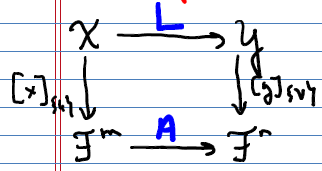
\includegraphics[width=0.42\columnwidth]{Chap02/DiagramChasingMatrixRep.png}}%
\hspace{5pt}%
\subfloat[]{%
	\centering
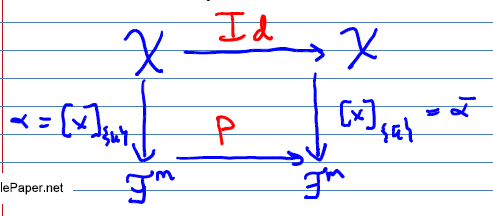
\includegraphics[width=0.52\columnwidth]{Chap02/DiagramChasingChangeOfBasis.png}}%
    \caption[]{Diagram chasing. Commuting diagrams used to illustrate the matrix representation of a linear operator and the change of basis matrix. When $\mathcal{X}=\mathcal{Y}$ and $\mathcal{L}=Id$, they become one and the same. Hence, there is really only one idea to remember.}
    \label{fig:DiagramChasing}
\end{figure} 

\vspace*{.2in}

\begin{example}
Let $\left(\mathcal{X},\mathcal{F}\right)=\left({\mathbb R}^{2},{\mathbb R}\right)$,
and define $L:{\mathbb R}^{2}\rightarrow{\mathbb R}^{2}$ by $L\left(e_{1}\right)=3e_{1}+4e_{2}$,
$L\left(e_{2}\right)=-e_{1}+6e_{2}$, where $e_{1}=\begin{bmatrix}1\\
0
\end{bmatrix}$ and $e_{2}=\begin{bmatrix}0\\
1
\end{bmatrix}$ are the canonical basis elements.
\begin{enumerate}
            \renewcommand{\labelenumi}{(\alph{enumi})}
        \setlength{\itemsep}{.1cm}
\item What is the matrix representation of $L$ with respect to $\left\{ e_{1},e_{2}\right\} $?
\item What is the matrix representation of $L$ with respect to $\left\{ v^{1},v^{2}\right\} $
where $v^{1}=e_{1}+e_{2}$, $v^{2}=3e_{1}-4e_{2}$?
\end{enumerate}
    
    \end{example}

\textbf{Solution:}~\begin{enumerate}
            \renewcommand{\labelenumi}{(\alph{enumi})}
        \setlength{\itemsep}{.1cm}
\item Let $A=$matrix representation of $L$. Then the $i^{th}$ column
of $A=\left[L\left(e_{i}\right)\right]_{\left\{ e_{1},e_{2}\right\} }$.
Hence,
\begin{align*}
\left[L\left(e_{1}\right)\right]_{\left\{ e_{1},e_{2}\right\} }&=\begin{bmatrix}3\\
4
\end{bmatrix} \\
\left[L\left(e_{2}\right)\right]_{\left\{ e_{1},e_{2}\right\} }&=\begin{bmatrix}-1\\
~~6
\end{bmatrix} \\
\implies A&=\begin{bmatrix}3 & -1\\
4 &~ ~6
\end{bmatrix}.
\end{align*}

\item Let $P$ be the change of coordinates from $\left\{ e_{1},e_{2}\right\} $
to $\left\{ v^{1},v^{2}\right\} $, and $\overline{P}$ be the change of
coordinates from $\left\{ v^{1},v^{2}\right\} $ to $\left\{ e_{1},e_{2}\right\} $.
Note that the $i^{th}$ column of $\overline{P}$ is just the representation
of $v^{i}$ in $\left\{ e_{1},e_{2}\right\} $. That is,
\[\overline{P}=\begin{bmatrix}1 & 3\\
1 & -4
\end{bmatrix}.\]
Recall that $\overline{P}=P^{-1}$, so
\[P=\left(\overline{P}\right)^{-1}=\frac{-1}{7}\begin{bmatrix}-4 & -3\\
-1 & 1
\end{bmatrix}=\frac{1}{7}\begin{bmatrix}4 & 3\\
1 & -1
\end{bmatrix}.\]
Therefore, if $\overline{A}$ is the representation of $L$ in $\left\{ v^{1},v^{2}\right\} $,
then
\[\overline{A}=PAP^{-1}=\frac{1}{7}\begin{bmatrix}4 & 3\\
1 & -1
\end{bmatrix}\begin{bmatrix}3 & -1\\
4 & 6
\end{bmatrix}\begin{bmatrix}1 & 3\\
1 & -4
\end{bmatrix}=\frac{1}{7}\begin{bmatrix}-38 & 16\\
-8 & 25
\end{bmatrix}.\]\\
\textbf{Note:} $\overline{P}$ was readily available, not $P$,
as you may have guessed!! Just to check, let's do the same thing the ``long way'':\\
\begin{align*}
L\left(v^{1}\right) & =L\left(e_{1}+e_{2}\right)\\
 & =L\left(e_{1}\right)+L\left(e_{2}\right)\\
 & =\left(3e_{1}+4e_{2}\right)+\left(-e_{1}+6e_{2}\right)\\
 & =2e_{1}+10e_{2}\\
L\left(v^{2}\right) & =L\left(3e_{1}-4e_{2}\right)\\
 & =3L\left(e_{1}\right)-4L\left(e_{2}\right)\\
 & =3\left(3e_{1}+4e_{2}\right)-4\left(-e_{1}+6e_{2}\right)\\
 & 13e_{1}-12e_{2}
\end{align*}
$\left[L\left(v^{1}\right)\right]_{\left\{ v^{1},v^{2}\right\} }=?$
To find it, write
\begin{align*}
\begin{bmatrix}2\\
10
\end{bmatrix} & =\overline{a}_{11}\underbrace{\begin{bmatrix}1\\
1
\end{bmatrix}}_{v^{1}}+\overline{a}_{21}\underbrace{\begin{bmatrix}3\\
-4
\end{bmatrix}}_{v^{2}}=\begin{bmatrix}1 & 3\\
1 & -4
\end{bmatrix}\begin{bmatrix}\overline{a}_{11}\\
\overline{a}_{12}
\end{bmatrix}\\
\implies & \begin{bmatrix}\overline{a}_{11}\\
\overline{a}_{12}
\end{bmatrix}=\frac{1}{7}\begin{bmatrix}38\\
-18
\end{bmatrix}
\end{align*}
Similarly
\begin{align*}
\begin{bmatrix}13\\
-12
\end{bmatrix} & =\overline{a}_{12}\begin{bmatrix}1\\
1
\end{bmatrix}+\overline{a}_{22}\begin{bmatrix}3\\
-4
\end{bmatrix}\\
\implies & \begin{bmatrix}\overline{a}_{12}\\
\overline{a}_{22}
\end{bmatrix}=\frac{1}{7}\begin{bmatrix}16\\
25
\end{bmatrix}
\end{align*}
and hence
$$ \overline{A}  =\frac{1}{7}\begin{bmatrix}38 & 16\\
-8 & 25
\end{bmatrix}. $$
\end{enumerate}

\Qed

\section{Eigenvalues, Eigenvectors, and Diagonalization}

\begin{definition}
Let $A$ be an $n\times n$ matrix with complex coefficients. A scalar $\lambda \in \mathbb{C} $ is an \textbf{eigenvalue} (e-value) of $A$, if there exists a non-zero vector $v \in \mathbb{C}^{n}$ such that $Av=\lambda v$. Any such vector $v$ is called an \textbf{eigenvector} (e-vector) associated with $\lambda$. 
\end{definition}

Eigenvectors are not unique because if $Av=\lambda v$, then for all $\alpha \neq 0$, $A(\alpha v)=\lambda (\alpha v)$, and thus $\alpha v$ is also an e-vector. To find eigenvalues, we need to know conditions under which $\exists v\neq0$ such that $Av=\lambda v$.
    \begin{equation*}
     \exists v\neq 0 \text{ s.t. }   Av=\lambda v \iff  \exists v\neq 0 \text{ s.t. } (\lambda I-A)v=0\iff \textnormal{det}(\lambda I-A)=0
    \end{equation*}
    
    \vspace*{.2cm}

\begin{example} Find the e-values and e-vectors for $A=\left[\begin{array}{rr}
    0 & 1\\
    -1 & 0
    \end{array}\right]$.
    \end{example} 
    
\textbf{Solution:}  $A=\left[\begin{array}{rr}
    0 & 1\\
    -1 & 0
    \end{array}\right] \implies \det(\lambda I-A)=\lambda^2+1=0$. Therefore, the eigenvalues are $\lambda_{1}=j,\lambda_{2}=-j$. To find eigenvectors, we need to solve $(A-\lambda_{i}I)v^{i}=0$. The eigenvectors are 
    $$v^{1}=\left[\begin{array}{c}
        1\\
        j
    \end{array}\right],v^{2}=\left[\begin{array}{c}
        1\\
        -j
    \end{array}\right].$$
Note that both eigenvalues and eigenvectors are complex conjugate pairs. 
\Qed




\begin{definition}
$\Delta (\lambda) := \det(\lambda I - A) $ is called the \textbf{characteristic polynomial}. $ \Delta (\lambda) = 0$ is called the \textbf{characteristic equation}. By the Fundamental Theorem of Algebra, $\Delta (\lambda)$ can be factored as
$$ \Delta (\lambda) = (\lambda - \lambda_1)^{m_1}(\lambda - \lambda_2)^{m_2}\dotsb(\lambda - \lambda_p)^{m_p} $$
where $\lambda_1, \dotsb, \lambda_p$ are the distinct eigenvalues (roots), $m_i$ is the \textbf{algebraic multiplicity} of $\lambda_i$, and  $m_1 + m_2 + \cdots + m_p = n.$ The \textbf{geometric multiplicity} of $\lambda i$ is defined as $\eta_i:= \dim \nullspace(A - \lambda_iI)$.

\end{definition}



\begin{thm}
Let $A$ be an $n \times n$ matrix with coefficients in $\real$ or $\mathbb{C}$. If the e-values $\{ \lambda_1,\ldots, \lambda_n \}$ are distinct, that is, $\lambda_i \neq \lambda_j $ for all $1 \le i \neq j \le n$, then the e-vectors $\{ v^1,\ldots,v^n \}$ are linearly independent in ($\mathbb{C}^n$,$\mathbb{C}$).
\end{thm} 

\begin{rem}
Restatement of the theorem: If the e-values $\{ \lambda_1,  \ldots,\lambda_n \}$ are distinct then $\{ v^1,  \ldots,v^n \}$ is a basis for ($\mathbb{C}^n$,$\mathbb{C}$).
\end{rem}

\textbf{Proof:}~We prove the contrapositive: if $\{ v^1,  \ldots,v^n \}$ is linearly dependent then there is a repeated e-value ($\lambda_i = \lambda_j$ for some $ i \neq j$). \\

$\{ v^1,  \ldots,v^n \}$ linearly dependent $\implies \exists$  $\alpha_1,  \ldots,\alpha_n \in \mathbb{C}$, not all zero, such that 
\begin{equation}
\label{eq:EvectorDependent}
     \alpha_1 v^1 + \dotsb + \alpha_n v^n = 0.
\end{equation}
   Without loss of generality, we can suppose $\alpha_1 \neq 0$. (that is, we can always reorder of e-values and e-vectors so that the first coefficient $\alpha_1$ is nonzero).\\
   
For all $1 \le i \le n$ and $1 \le j \le n$, because $v^i$ is an e-vector,
$$(A - \lambda_j I)v^i = A v^i - \lambda_j v^i = \lambda_i v^i - \lambda_j v^i = (\lambda_i - \lambda_j) v^i.$$

Using this fact, it is an easy exercise to show 
\begin{equation}
\label{eq:ProductMatrices}
(A - \lambda_2 I)(A - \lambda_3 I)\dotsb(A - \lambda_n I)v^i = (\lambda_i - \lambda_2)(\lambda_i - \lambda_3)\dotsb(\lambda_i - \lambda_n)v^i, \text{ for  } 1 \leq i \leq n.
\end{equation}
Plugging in now for $i$ yields,\\

   for $i = 1$ $$ (A - \lambda_2 I)(A - \lambda_3 I)\dotsb(A - \lambda_n I)v^1 = (\lambda_1 - \lambda_2)(\lambda_1 - \lambda_3)\dotsb(\lambda_1 - \lambda_n)v^1; \hspace*{4.1cm}$$
    for $i = 2$ $$(A - \lambda_2 I)(A - \lambda_3 I)\dotsb(A - \lambda_n I)v^2= (\lambda_2 - \lambda_2)(\lambda_2 - \lambda_3)\dotsb(\lambda_2 - \lambda_n)v^2 = 0 \text{ because } (\lambda_2 - \lambda_2)=0;$$
    $$ \vdots$$
for $i = n$ $$ (A - \lambda_2 I)(A - \lambda_3 I)\dotsb(A - \lambda_n I)v^n = (\lambda_n - \lambda_2)(\lambda_n - \lambda_3)\dotsb(\lambda_n - \lambda_n)v^2 = 0 \text{ because } (\lambda_n - \lambda_n)=0. $$



    Combining the above with \eqref{eq:EvectorDependent}, we obtain
    \begin{align*}
        0 &= (A - \lambda_2 I)(A - \lambda_3 I)\dotsb(A - \lambda_n I)(\alpha_1 v^1 + \dotsb + \alpha_n v^n)\\
        & = \alpha_1 (\lambda_1 - \lambda_2)(\lambda_1 - \lambda_3)\dotsb(\lambda_1 - \lambda_n)v^1
    \end{align*}

    We know $\alpha_1 \neq 0$, as stated above, and $v^1 \neq 0$, by definition of e-vectors. Therefore, 
    $$0 = (\lambda_1 - \lambda_2)(\lambda_1 - \lambda_3)\dotsb(\lambda_1 - \lambda_n),$$
    and hence, at least one of the terms $(\lambda_1-\lambda_k)$, $2 \le k \le n$ must be zero. Therefore, there is a repeated e-value $\lambda_1 = \lambda_k $ for some $2 \leq k \leq n$. 
    \Qed



\vspace*{.2cm}

\section{A Few Additional Properties of Matrices}

\vspace*{.2cm}

\begin{definition}
Two $n \times n$ matrices $A$ and $B$ are \textbf{similar} if there exists an invertible $n \times n$ matrix $P$ such that $B=P \cdot A \cdot P^{-1}$. $P$ is called a \textbf{similarity} matrix. 
\end{definition}

\begin{definition}
An $n \times n$ matrix $A$ is said to have a \textbf{full set of e-vectors} if there exists a basis $\{ v^1, v^2, \ldots, v^n\}$ of $(\cp^n, \cp)$ such $A v^i = \lambda_i v^i$, $1 \le i \le n$.
\end{definition}

\begin{thm}
\label{thm:SimilarDiagnonalMatrix}
An $n \times n$ matrix $A$ has a full set of e-vectors if, and only if, it is similar to a diagonal matrix. And when this happens, the entries on the diagonal matrix are e-values of $A$.
\end{thm} 

\textbf{Proof:} We assume that $\{ v^1, \ldots, v^n \}$ is a basis for $(\cp^n, \cp)$ and that for $1 \le i \le n$, $A v^i = \lambda_i v^i$. Define two $n \times n$ matrices
\begin{align*}
    M &:= \left[ \begin{array}{cccc} v^1 & v^2 & \cdots & v^n \end{array} \right] \\
    \Lambda &:= {\rm diag}(\lambda_1, \lambda_2, \ldots, \lambda_n).
\end{align*}
Then 
\begin{align*}
   A \cdot M &:= \left[ \begin{array}{cccc} A v^1 & A v^2 & \cdots & A v^n \end{array} \right] \\
   &=\left[ \begin{array}{cccc} \lambda_1 v^1 & \lambda_2 v^2 & \cdots & \lambda_n v^n \end{array} \right] \\
  &= M \cdot \Lambda.
\end{align*}
 
 We'll leave as an Exercise, 
 $$ M  \alpha = \left[ \begin{array}{cccc} v^1 & v^2 & \cdots & v^n \end{array} \right]  \begin{bmatrix}\alpha_{1}\\
            \alpha_{2}\\
            \vdots\\
            \alpha_{n}
        \end{bmatrix} = \alpha_1 v^2 + \alpha_2 v^2 + \cdots + \alpha_n v^n,$$
        and hence $M$ is invertible if, and only if, $\{ v^1, \ldots, v^n \}$ is linearly independent. Therefore we have 
        $$A = M \Lambda M^{-1} \text{ and } \Lambda = M^{-1} A M, $$
        proving that  $\{ v^1, \ldots, v^n \}$ is a basis implies $A$ is similar to a diagonal matrix. \\
        
        The other direction is straightforward and left to the reader. You need to recognize the columns of the ``similarity matrix'' as being e-vectors of $A$.
\Qed

\begin{fact}
If $A$ and $B$ are similar, they have the same e-values. Moreover, the e-values have the same algebraic and geometric multiplicities. 
\end{fact} 



\begin{definition}
 Let $A$ be an $n \times m$ matrix with coefficients in $\real$ or  $\cp$. The \textbf{rank} of $A$ is equal to the number of linearly independent columns. 
\end{definition}

\begin{fact}
If $M$ is square, then $\rank(M)$ equals the number of non-zero e-values.
\end{fact}

\begin{fact}
\label{fact:rankAAtranspose}
For an $n \times m$ real matrix $A$, $\rank(A) = \rank(A^\top A) = \rank(AA^\top) = \rank(A^\top)$. Hence, $A^\top A$ and $AA^\top$ have the same number of non-zero e-values. For a proof, see Chapter 10 of the ROB 101 textbook and see Lemma~\ref{lem:EigenStuffAAtranspose} below.
\end{fact} 




\begin{cor}\mbox{ }
\begin{itemize}
    \item $\#$ of linearly independent rows  = $\#$ of linearly independent columns.
    \item $\rank(A) \le \min(n, m)$
\end{itemize}
\end{cor}

\begin{lem}
\label{lem:EigenStuffAAtranspose}
Suppose that $A$ is a real $n \times m$ matrix. Then, 
\begin{itemize}
    \item If $\lambda$ is a non-zero e-value of $\left(A^\top A \right)$ with e-vector $v$, then $\lambda$ is also an e-value of $\left(A A^\top \right)$ with e-vector $A v$.
    \item If $\lambda$ is a non-zero e-value of $\left(A A^\top \right)$ with e-vector $v$, then $\lambda$ is also an e-value of $\left( A^\top A \right)$ with e-vector $A^\top  v$.
\end{itemize}
\end{lem}

\textbf{Proof:} We only prove the first statement. Suppose that $\left(A^\top A \right)v = \lambda v$ and both $\lambda$ and $v$ are non-zero. Then $Av \neq 0$. Next, we form 
$$\left(A A^\top \right) \left(A v \right)= A  \left( A^\top A\right)  v = A \left(\lambda v\right) = \lambda \left(Av\right),$$ 
and thus $\lambda$ is an e-value of $\left(A A^\top \right)$ with e-vector $Av$.

\Qed

\begin{cor} $A A^\top$ and $A^\top A$ have the same non-zero e-values. Because they have different sizes, they may have different number of zero e-values. 
\end{cor}

\begin{definition}(\textbf{Trace of a Matrix}) Let $C$ be an $n \times n$ matrix. Then $\tr(C):=\sum_{i-1}^n C_{ii}.$
\end{definition}

\begin{exercise} Suppose that $A$ is $n \times m$ and $B$ is $m \times n$. Then
$$\tr(A\cdot B) = \tr(B \cdot A). $$

\end{exercise}

 
\begin{fact}
\label{fact:MatMultiplyAlternative}
\textbf{(A lesser known way doing matrix multiplication, the outer product formula.)}  Suppose that $A$ is $n \times k$ and $B$ is $k \times m$ so that the two matrices are compatible for matrix multiplication. Then 
$$A\cdot B = \sum_{i=1}^{k} a_i^{\rm col} \cdot b_i^{\rm row},  $$
the ``sum of the columns of $A$ multiplied by the rows of $B$''. A more precise way to say it would be ``the sum over $i$ of the $i$-th column of $A$ times the $i$-th row of $B$.'' 
\end{fact}

\textbf{Why:} To see why this is true, let's first consider two $2 \times 2$ matrices $A$ and $B$, where
$$A= \left[\begin{array}{cc} a_{11}& a_{12} \\ a_{21} & a_{22}\end{array}\right]
\text{ and } B= \left[\begin{array}{cc} b_{11}& b_{12} \\ b_{21} & b_{22}\end{array}\right]
.$$
Then, using the standard rows of $A$ times the columns of $B$ formulation of matrix multiplication yields
$$
\begin{aligned}
 A \cdot B := &
\left[\begin{array}{cc}  a_1^{\rm row} \cdot b_1^{\rm col} & a_1^{\rm row} \cdot b_2^{\rm col}  \medskip  \\
a_2^{\rm row} \cdot b_1^{\rm col} & a_2^{\rm row} \cdot b_2^{\rm col}
\end{array}\right] \\ 
=& \left[\begin{array}{cc}  a_{11} b_{11} + a_{12}b_{21} & a_{11} b_{12} + a_{12}b_{22} \\
a_{21} b_{11} + a_{22}b_{21} & a_{21} b_{12} + a_{22}b_{22}
\end{array}\right]\bigskip  \text{(next, we take the sum outside the matrix)}\\
=& \left[\begin{array}{cc}  a_{11} b_{11}  & a_{11} b_{12} \\
a_{21} b_{11}  & a_{21} b_{12} 
\end{array}\right] + \left[\begin{array}{cc}  a_{12} b_{21}  & a_{12} b_{22} \\
a_{22} b_{21}  & a_{22} b_{22} 
\end{array}\right] \bigskip  \text{(next, we recognize each term)}\\
=& \left[\begin{array}{c} a_{11}\\ a_{21} \end{array}\right] \cdot 
 \left[\begin{array}{cc} b_{11}& b_{12} \end{array}\right] + 
 \left[\begin{array}{c} a_{12}\\ a_{22} \end{array}\right] \cdot 
 \left[\begin{array}{cc} b_{21}& b_{22} \end{array}\right]\\
=& a^{\rm col}_1 \cdot b^{\rm row}_1 + a^{\rm col}_2 \cdot b^{\rm row}_2
\end{aligned}
$$

In a similar manner, we can treat the general case,
\begin{equation}
\begin{aligned}
   A \cdot B:=&  \left[\begin{array}{c}\boxed{a_{11}~~ a_{12}~~ \cdots~~ a_{1k}}  \medskip \\
\boxed{a_{21}~~ a_{22}~~ \cdots~~ a_{2k}} \\
\vdots \\
\boxed{a_{n1}~~ a_{n2}~~ \cdots~~ a_{nk}}\end{array}\right] \cdot 
\left[ \boxed{\begin{array}{c} b_{11} \\ b_{21}\\ \vdots \\ b_{k1}\end{array} }~~~
\boxed{\begin{array}{c} b_{12} \\ b_{22}\\ \vdots \\ b_{k2}\end{array} }~~~\cdots~~~
\boxed{\begin{array}{c} b_{1m} \\ b_{2m}\\ \vdots \\ b_{km}\end{array} }\right] \\
=&
%
\left[\begin{array}{cccc}  \sum\limits_{i=1}^k a_{1i}b_{i1} & \sum\limits_{i=1}^k a_{1i}b_{i2} & \cdots & \sum\limits_{i=1}^k a_{1i}b_{im}  \medskip \\
 \sum\limits_{i=1}^k a_{2i}b_{i1} & \sum\limits_{i=1}^k a_{2i}b_{i2} & \cdots & \sum\limits_{i=1}^k a_{2i}b_{im} \\
\vdots & \vdots & \ddots & \vdots \\
 \sum\limits_{i=1}^k a_{ni}b_{i1} & \sum\limits_{i=1}^k a_{ni}b_{i2} & \cdots & \sum\limits_{i=1}^k a_{ni}b_{im} \\
\end{array}\right] \text{ (next, we pull the sum outside the matrix)}\\
=& \sum\limits_{i=1}^k
\left[\begin{array}{cccc}   a_{1i}b_{i1} &a_{1i}b_{i2} & \cdots &  a_{1i}b_{im}  \medskip \\
     a_{2i}b_{i1} & a_{2i}b_{i2} & \cdots &  a_{2i}b_{im} \\
\vdots & \vdots & \ddots & \vdots \\
  a_{ni}b_{i1} & a_{ni}b_{i2} & \cdots &  a_{ni}b_{im} \\
\end{array}\right] \text{(next, we recognize what this is)}\\
=& \sum_{i=1}^{k} a_i^{\rm col} \cdot b_i^{\rm row} \\
=&
\left[ \boxed{\begin{array}{c} a_{11} \\ a_{21}\\ \vdots \\ a_{n1}\end{array} }~~~
\boxed{\begin{array}{c} a_{12} \\ a_{22}\\ \vdots \\ a_{n2}\end{array} }~~~\cdots~~~
\boxed{\begin{array}{c} a_{1k} \\ a_{2k}\\ \vdots \\ a_{nk}\end{array} }\right] \cdot  \left[\begin{array}{c}\boxed{b_{11}~~ b_{12}~~ \cdots~~ b_{1m}}  \medskip \\
\boxed{b_{21}~~ b_{22}~~ \cdots~~ b_{2m}} \\
\vdots \\
\boxed{b_{k1}~~ b_{k2}~~ \cdots~~ b_{km}}\end{array}\right]. \
\end{aligned}
\end{equation}
\Qed


\begin{fact} \textbf{(Matrix Inversion Lemma)} Suppose that $A$, $B$, $C$ and $D$ are compatible\footnote{The sizes are such the matrix products and sum in $A+BCD$ make sense.} matrices. If $A$, $C$, and  $(C^{-1}+D A^{-1}B)$ are each square and invertible, then  $A+BCD$ is invertible and
    $$ (A + BCD)^{-1} = A^{-1} - A^{-1}B(C^{-1} + DA^{-1}B)^{-1}DA^{-1}$$
\end{fact}

\begin{rem} In many important applications, the inverse of $A$ may be already known or easy to compute. Here is a made up example, but it gets the point across: By hand, evaluate $ (A + BCD)^{-1}$ when
        $$A=\mathrm{diag}([1,~0.5, ~0.5,~1,~ 0.5]), ~ B=\begin{bmatrix} 1 \\ 0\\ 2\\ 0 \\3 \end{bmatrix}, C=0.2, D= B^\top $$
\end{rem}



